\documentclass[twocolumn]{article}

\usepackage[utf8]{inputenc}
\usepackage[T2A]{fontenc}
\usepackage[utf8]{inputenc}
\usepackage[russian]{babel}
\usepackage[margin=0.7in]{geometry}
\usepackage{hyperref}
\usepackage{xspace}
\usepackage{xcolor}
\usepackage{graphicx}
\usepackage{indentfirst}
\graphicspath{ {./pictures/} }

\title{Grimdark Future}

\newcommand{\dicespan}[2]{\mbox{#1-#2}}
\newcommand{\h}[1]{\textbf{#1}}
\newcommand{\D}[1][6]{D#1\xspace}
\newcommand{\TODO}{\begin{center}\color{red}TODO\end{center}}
\newcommand{\ssec}[1]{\section{#1}\label{sec:#1}}
\newcommand{\subsec}[1]{\subsection{#1}\label{subsec:#1}}
\newcommand{\subsubsec}[1]{\subsubsection{#1}\label{subsubsec:#1}}

\pagenumbering{gobble}
\begin{document}

\maketitle
\tableofcontents

\newpage

\ssec{Общие Принципы}
\subsec{Что происходит?}
Игроки берут на себя роли командиров одной или нескольких конфликтующих армий и решительно ведут их в бой. Битва состоит из поочерёдных ходов, в течение каждого из которых игроки передвигают свои армии, атакуют и прочими способами пытаются осла- бить силы противника параллельно выполняя миссии - задачи своей армии. Кто набрал обговоренное количество победных очков или лишил противника возможности набрать достаточное выигрывает.

\subsec{Как читать эти правила?}
Желательно, по порядку. Если вы читаете этот пункт, вы скорее всего уловили суть происходящего и вопросы связаны со спецификой, так что читайте по порядку.

\subsec{Общие Термины}
Юнит это общее название для одной боевой единицы. Юнитом может быть как отряд из двадцати солдат с винтовками, так и одинокий мощный танк. Модель это один солдат из юнита.

\subsec{Самое Главное Правило}
Как и в любой сложной игре будут ситуации, не предусмотренные правилами или правила неоднознач- ны. Когда такое происходит, действуйте так, как подсказывает здравый смысл или личные предпочтения. Если же игроки не могут решить, как должно действовать определённое правило в конкретной ситуации, используйте следующий метод: Бросьте кубик. Если выпадает 1-3, то правило действует так, как решил иг- рок А, если выпадает 4-6, то решает игрок Б.

\subsec{Масштаб и Размеры}
Правила игры сделаны для круглых подставок диаметром 28мм, но при желании можно обойтись и без них. Если же подставок нет могут возникнуть сложности с измерением расстояний. Если игроки не готовы терпеть неоднозначность измерений либо оспаривается спорная ситуация, предлагается измерить расстояние от центра моделей и вычесть подходящие радиусы подставок. Некоторые модели требуют подставки других размeров, рекомендуется придерживаться следующих диаметров для моделей соответвующих типов:

\begin{itemize}
    \item \h{Пехота}: от 20мм до 40мм
    \item \h{Мотоциклы и Твари}: 25мм X 70мм
    \item \h{Монстры и Тяжёлая Техника}: 60мм
    \item \h{Транспорт}: без подставки
\end{itemize}

\subsec{Параметры Юнита}
К юнитам приложено множество параметров, определяющих кто они и что могут делать.

\begin{itemize}
    \item \h{Название [Кол-во]}: Имя юнита и количество мо- делей. Например "Терминаторы [4]" означает отряд из четырёх терминаторов, вместе считаемых одним юнитом.
    \item \h{Мощь}: Бросок для проверок атаки и боевого духа. Это условная характеристика силы каждого отряда.
    \item \h{Защита}: Бросок для проверок защиты. Насколько хорошо этот отряд может переживать выстрелы и снаряды. Высокие показатели могут ассоциироваться как с высокой ловкостью, так и с высокой бронированностью.
    \item \h{Экипировка}: Oружие, которыми обладает этот юнит. Оно определяет все конкретные атаки, производимые юнитом и чаще всего даётся на выбор игрокам. Оружие также часто имеет особые правила.
    \item \h{Особые Правила}: равила, которые применяются к этому юниту. Некоторые юниты способны быстро пересекать трудную местность, другие могут надёжно пробивать вражескую броню.
    \item \h{Стоимость}: Стоимость этого юнита в поинтах, почти всегда прямопропорциональная его общей боевой сиде. Поинты используются для распределения цены армий, например в битве на 2500 поинтов с обоих сторон выступают армии с суммарной ценой 2500 поинтов или чуть ниже. 
\end{itemize}

\subsec{Кубы и Броски}
Для игры требуется несколько шестигранных кубов, далее \D[6]. В зависимости от количества моделей на столе рекомендуется иметь от 10 до 20 кубов, также предлагается иметь кубы разной расцветки для ускорения игрового процесса, когда юнит одновременно совершает броски разных типов.

Иногда правила требуют разные кубы, например \D[3], 2\D и \D+1. Для понимания этой формы записи просто пользуйтесь следующими правилами:

\begin{itemize}
    \item \h{\D[3]}: Чтобы узнать значение используйте \D, результат разделите пополам и округлите вверх (напр. 6 на \D  это 3 на \D[3], а 3 на \D это 2 на \D[3])
    \item \h{2\D}: Чтобы узнать значение бросьте два куба и проссумируйте значения на каждом.
    \item \h{\D[6]+1}: Чтобы узнать значение, бросто бросьте кубик и прибавьте к результату единицу.
\end{itemize}

\subsec{Переброс (англ. Re-Roll)}
Когда правило предлагает вам перебросить куб, вы повторно совершаете бросок. Выпавший результат считается финальным, даже если он хуже предыдущего. \emph{Каждый куб можно перебросить только один раз, независимо от того, сколько правил на него действуют.}

\subsec{Столкновение (англ. Roll-Offs)}
Когда правило требует столкновение, все участные игроки совершают бросок и сравнивают результаты. Игрок с наибольшим считается победителем. В случае ничьи игроки должны повторить столкновение, пока не будет определён однозначный победитель.

\subsec{Проверка Мощи}
В течение игры иногда будет необходимо провести проверку мощи, чтобы узнать как юнит справится с атакой противника или поддержкой боевого духа. Если правило требует проверку мощи, бросьте один куб. Если результат совпадает или превышает параметр мощи юнита, проверка считается пройденной, иначе - проваленой.

\subsec{Модификаторы}
В течение игры некоторые правила предлагают изменить результат броска, обычно повысить или убавить значение на единицу, но конкретные числа могут различаться. Применяя модификатор увеличьте или уменьшите значение на нужное число. \emph{Независимо от модификаторов 1 всегда считается провалом, а 6 - успехом.}

\subsec{Оружие}
Все оружия в игре делятся на две категории: ближнего и дальнего боя. Оружия дальнего боя обладают параметром дальности, используемым для стрельбы, оружия ближнего - нет. Оружия представлены следуюищим образом:
\begin{center}
    \textit{Название (Дальность, Атака, Особые Правила)}
\end{center}

\subsec{Расстояния}
Для игры вам потребуется линейка, расстояние измеряется от края подставки, если край подставки отсутсвует - измеряйте от крайней разумной точки. При измерении растояний между двумя моделями, измеряется расстояние от/до края подставки. При измерении расстояния между юнитами, измеряется расстояние между двумя ближайшими моделями. При перемещении самая дальнаяя часть модели не может оказаться дальше чем общее расстояние перемещения.

\subsec{Видимость}
Если не указано иначе, каждая модель видит во всех направлениях. Чтобы определить видит ли одна модель другую проведите прямую между видящим и видимой моделью. Если прямая не пересекает сплошных препятствий (включая другие юниты), модель находится в области видимости. \emph{Модели того же юнита не учитываются при измерениях.}

\vspace{24pt}
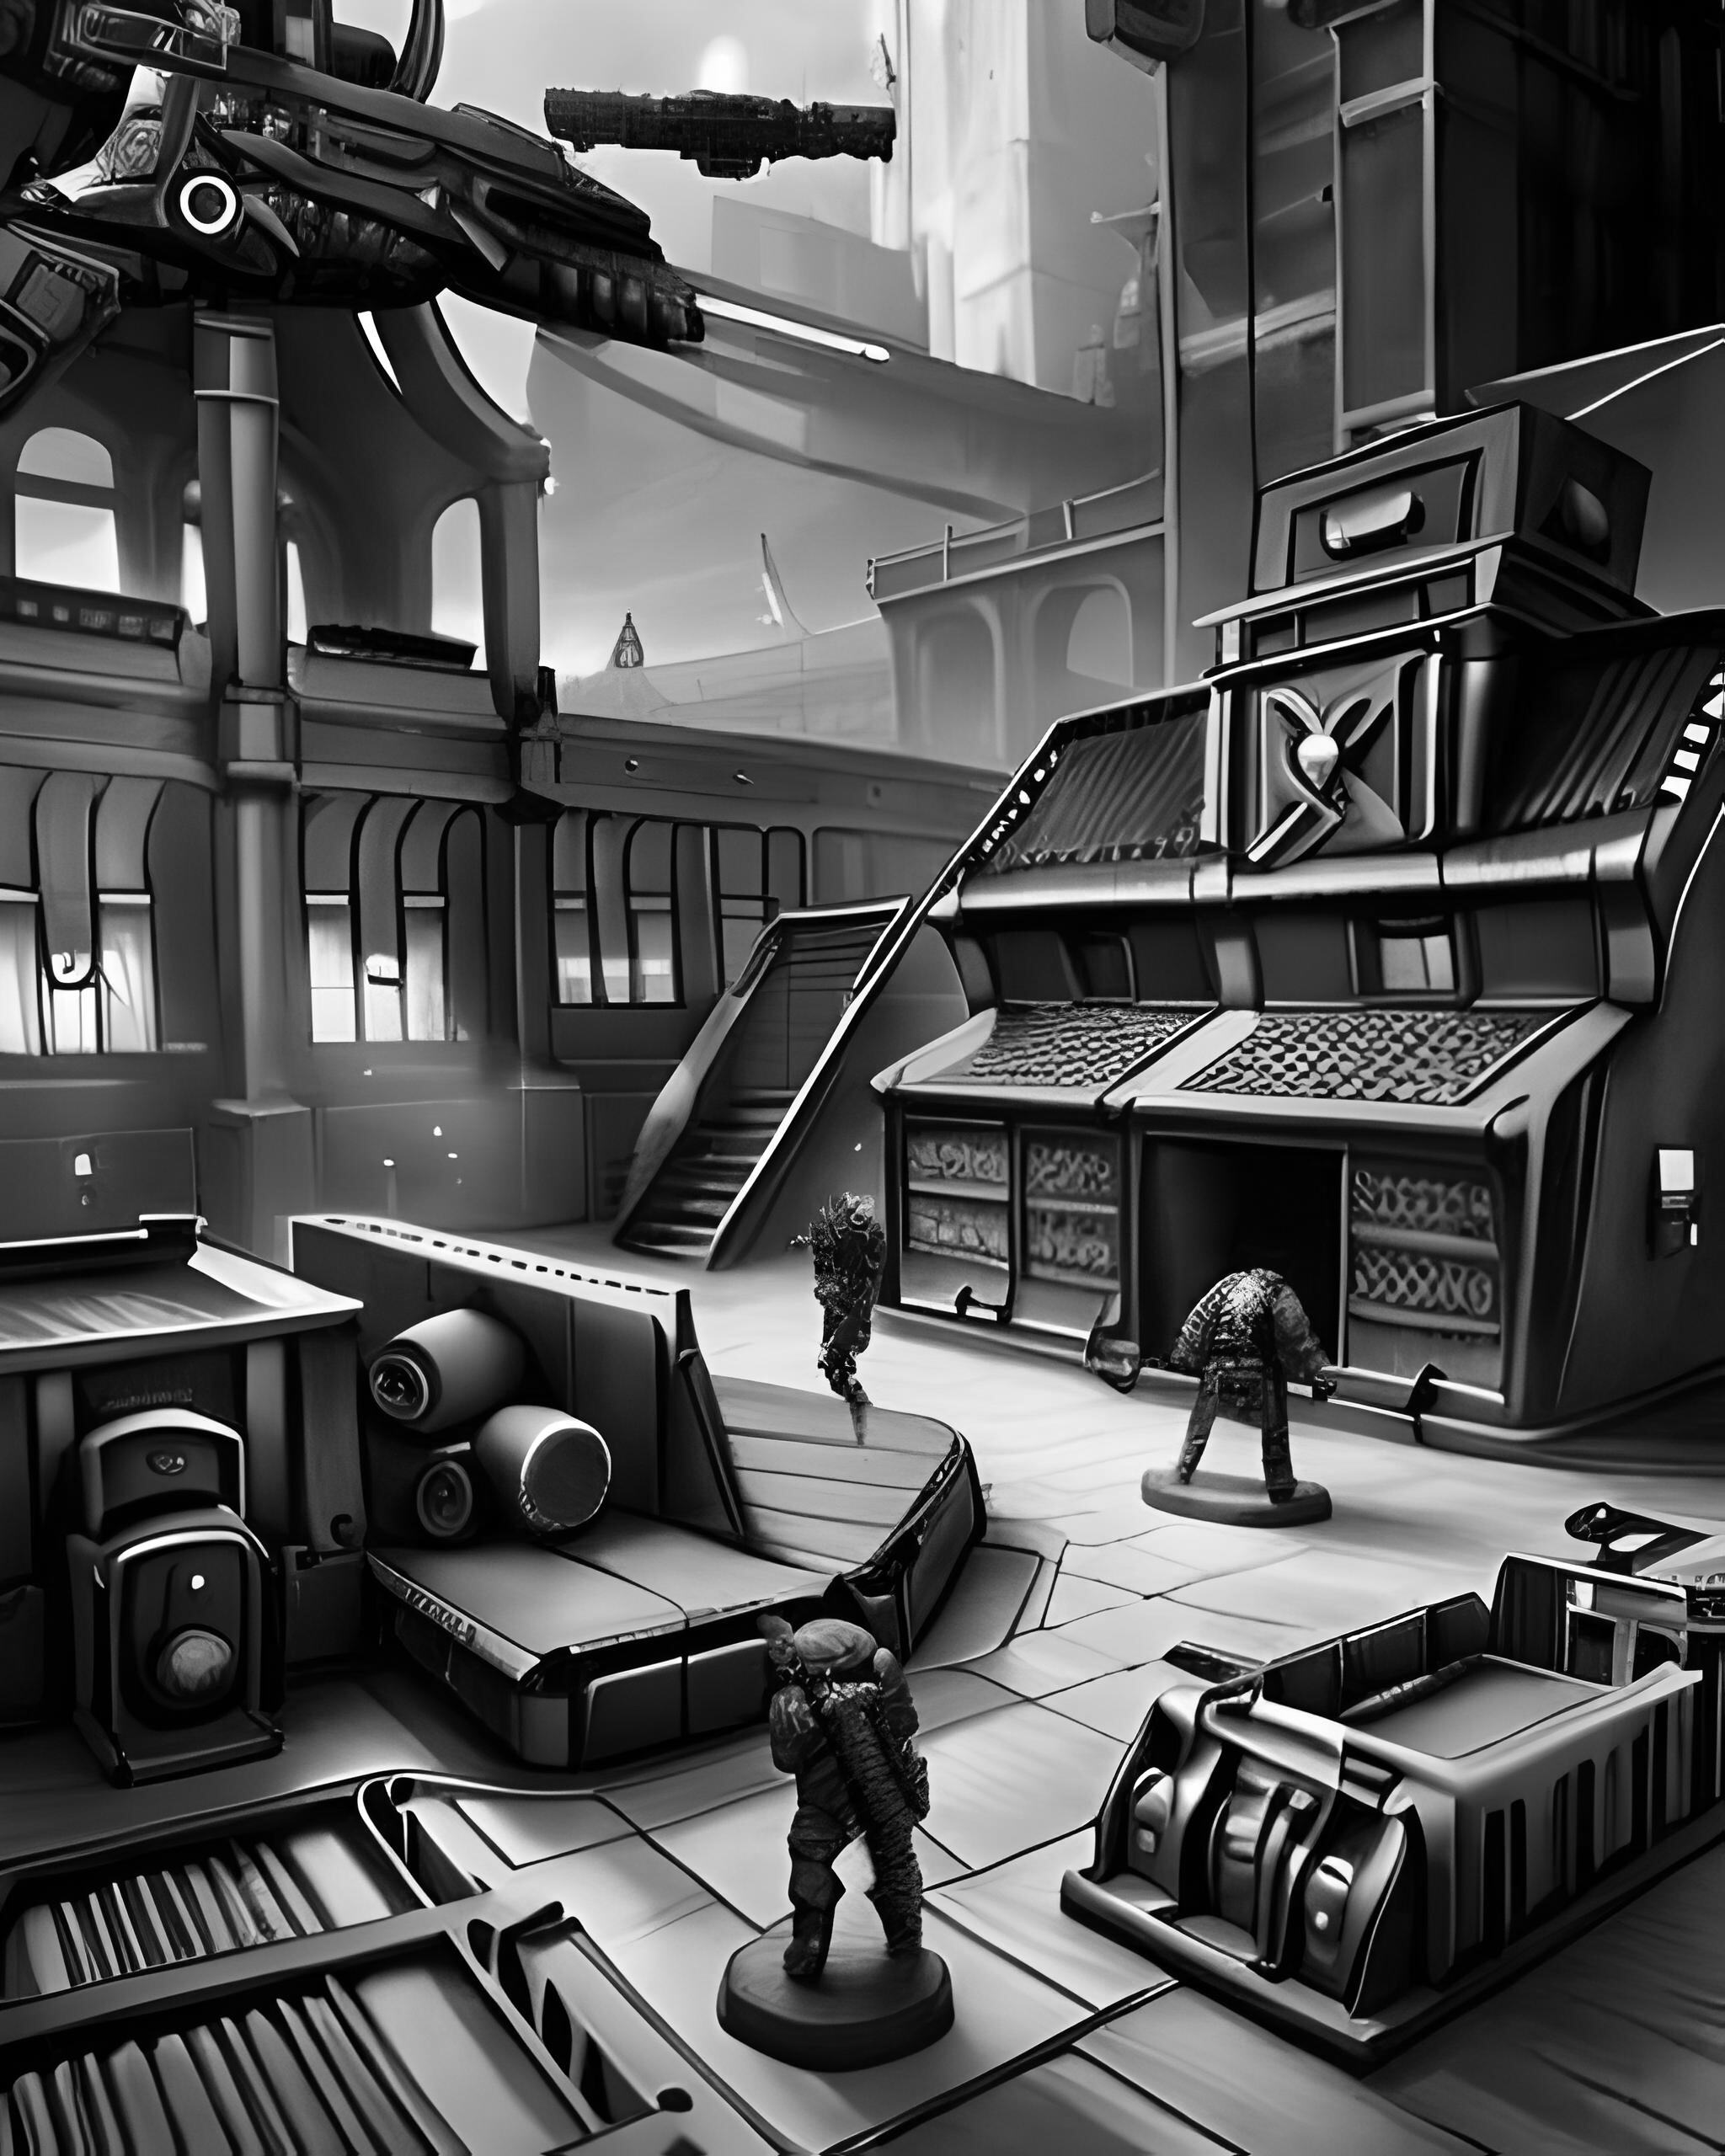
\includegraphics[width=0.9\columnwidth]{Strategy}

\newpage

\ssec{Подготовка}
\subsec{Поле боя}
Вам потребуется игровая поверхноть, будь то пол комнаты, стол или даже кровать. Эта поверхность далее называется "поле боя" или же просто "игровой стол".

Когда вы нашли себе игровое пространство, можно расставить преграды и части местности. Рекомендуется использовать от 10 до 15 (а в некоторых случаях и более) преград. Поскольку отсутсвуют конкретные правила расстановки особенностей местности рекомендуется самостоятельно контролировать сбалансированность. Оптимально расставить местность так, чтобы две модели на противоположных концах стола не могли видеть друг друга, а также, при возможности, избежать пропостей между частями местности более чем 30 см.

\subsec{Выбор Сценария}
Сценарий определяет условия и художественные обстоятельства происходящей битвы. Это включает области высадки, возможные препятствия, природные катаклизмы и тому подобное. Список доступен в соответвующем разделе.

\subsec{Выбор Миссиий}
Игроки расставляют на поле 6 тактических маркеров на поле по очереди. Очерёдность выставления определяется столкновением. Тактические маркеры должны быть на расстоянии 25см друг от друга и от границ зон высадки. Далее игроки смотрят на таблицу миссий и выбирают. Каждый игрок в момент выбора может должен взять себе одну из доступных миссий, а затем запретить оппоненту одну из оставшихся. Это продолжается пока игроки не наберут миссий, в сумме дающих оговоренное количество победных очков.

\subsec{Сбор Армии}
Перед началом игры вы и ваш противник должны определиться с размером отрядов. Для начала рекомендуется иметь армии по 750 поинтов, позже можно перейти к более тяжёлым армиям. Чтобы собрать армию просто выберите модели, юнитов, улучшения для них и убедитесь что сумма поинтов не превышает обговоренного числа. Количество юнитов не ограничено ничем кроме максимального количества поинтов.

\subsec{Комбинированные Юниты}
При подготовке армии вы можете совместить два малых юнита в один больший, при условии что у них не отличается список улучшений.

\subsec{Высадка}
Когда все условия для подготовки миссии исполнены, игроки начинают выставлять своих юнитов. Совершите столкновение между всеми выставляющими, победитель определяет порядок высадки. В этом порядке каждый игрок ставит одного юнита в своей зоне высадки (таковая описана в подробностях миссии). Это продолжается пока не выставлены все юниты.

\newpage

\ssec{Ход Игры}
\subsec{Раунды, Ходы и Активации}
Игра разделена на раунды, ходы игроков и активации юнитов:
\begin{itemize}
    \item \h{Раунд}: Каждый раунд состоит из нескольких ходов
    \item \h{Ход}: Каждый ход состоит из одной активации
    \item \h{Активация}: Каждая активация состоит из одного действия
\end{itemize}

\subsec{Структура Игры}
После того как оба игрока высадили свои армии начинается первый раунд. Игрок, победивший при определении порядка высадки также определяет порядок хода. В свой ход игрок выбирает юнита, который ещё не был активирован и активирует его, совершая действие. Как только действие выполнено, ход заканчивается и передаётся следующему игроку. Это продолжается пока все юниты не будут активированы, в этот момент раунд заканчивается и начинается следующий. Следующий раунд начинает следующий человек в порядке хода. Условие окончания игры обозначено в миссии.

\subsec{Сплочённость Юнитов}
Юниты состоят из двух и более моделей, которые обязаны соблюдать правило сплочённости.
Все модели в юните обязаны находиться в радиусе 5 см и меньше от любой другой модели из юнита и в радиусе 15 см и меньше от всех других моделей в юните.
Если в начале активации одна из моделей отсоединена от остального юнита, то она обязана совершить действие, передвигающие модель для соблюдения этого правила.

\subsec{Активация Юнита}
Игроки могут активировать одного юнита, который ещё не был активирован и исполнить одно действие:
\begin{itemize}
    \item \h{Оборона}: Юнит может стрелять и остаётся на месте и может стрелять.
    \item \h{Продвижение}: Юнит двигается на расстояние до 15 см и может стрелять после передвижения.
    \item \h{Рывок}: Юнит двигается на расстояние до 30 см и не может стрелять.
    \item \h{Прорыв}: Юнит двигается на расстояние до до 30 см, чтобы войти в расстояние ближнего боя с противником. Юнит не может стрелять. Юнит может атаковать только если хоть одна модель может войти в ближний бой.
\end{itemize}

\newpage

\subsubsec{Оборона}
Когда юнит обороняется, все модели в нём не могут повернуться или двинуться.

\subsubsec{Продвижение}
Продвигаясь, все модели в юните могут передвинуться на вплоть до 15 см. Расстояние передвижения в финальном положении измеряется от той же точки модели, от которой оно измерялось в начале движения. (напр. если передвижение планировалось от края подставки, то конец движения измеряется \emph{от того же} края подставки).

Моделям не разрешается пододвигаться к другим моделям (вражеским или дружеским) ближе чем на 1 см.

\emph{Модели не могут двигаться сквозь другие модели.}

\subsubsec{Рывок}
Совершая рывок, все модели в юните могут передвинуться на вплоть до 30 см. Применяются те же ограничения, что и при продвижении (движение сквозь, 1 см расстояния от других моделей).

\subsubsec{Прорыв}
Прорываясь, все модели в юните могут передвинуться на вплоть до 30 см. \emph{Модели не могут двигаться сквозь другие модели, но могут игнорировать ограничение на минимальное расстояние в 1 см. Более подробно далее, в отделе про ближний бой. Юнит может совершить прорыв если хоть одна модель сможет войти в ближний бой с противником.}

\subsec{Боевой Дух}
После столкновения (в дальнем или ближнем бою) подсчитывается количество ран, нанесённых обоим юнитам. В случае ближнего боя проверку боевого духа совершает юнит, понёсший наибольшее количество потерь (при ничье проверку проводят обе стороны), в случае дальнего - обе. \emph{Если отряд не понёс потерь он не обязан проводить проверку.} Юнит обязан провести проверку боевого духа, если потерял больше половины моделей за один ход.

\vspace{12pt}
\begin{center}
    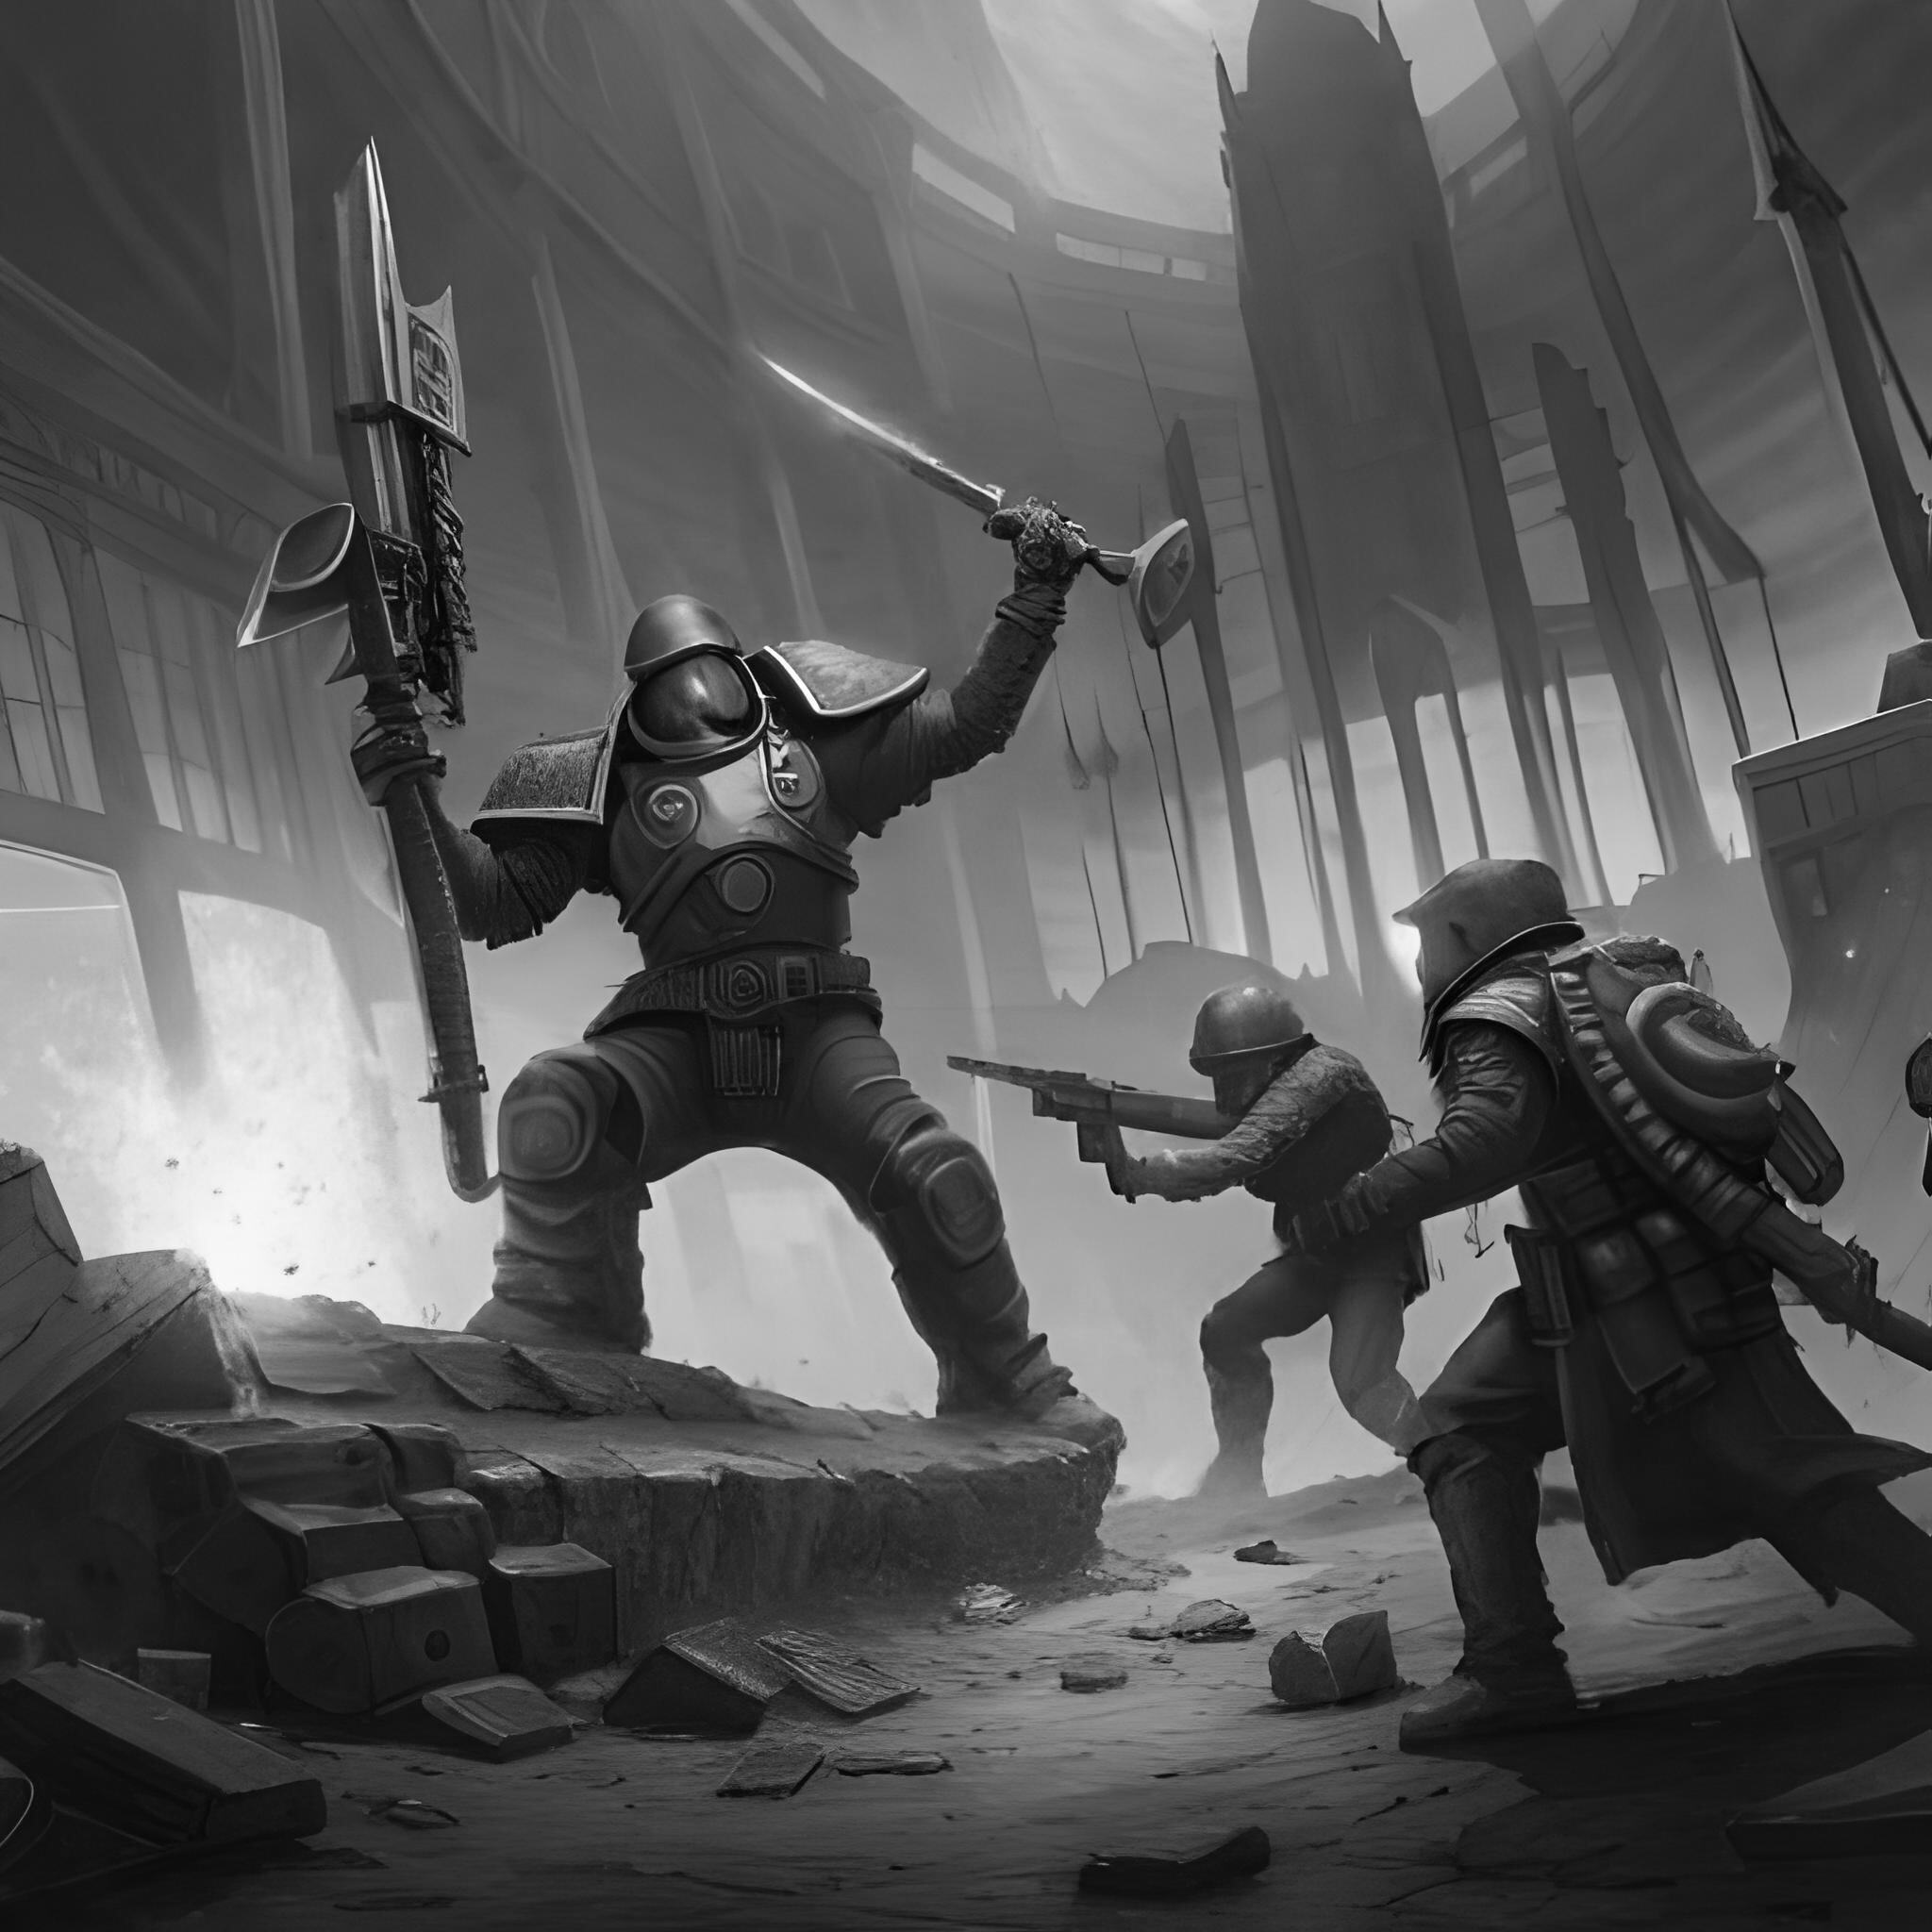
\includegraphics[width=0.5\columnwidth]{Perseverance}
\end{center}

\newpage

\ssec{Стрельба}
\subsec{Выбор Целей}
Стреляя, юнит должен выбрать один другой досягаемый юнит как цель, все модели могут в неё стрелять.
Цель считается досягаемой, если она является видимой хоть для одной модели и цель находится в радиусе досягаемости оружия этого юнита.
\subsec{Разное Оружие}
Если юнит имеет несколько разных оружий, можно разделить его на несколько групп, по оружию на группу. Каждая группа может выбрать свою цель. Все модели в группе обязаны стрелять по одной цели. \emph{Цель для каждой группы должна быть объявлена до бросков. Считается что все группы стреляют одновременно.}

\subsec{Открыть Огонь!}
Стрельба включает в себя 4 шага:
\begin{itemize}
    \item \h{Определение атак}: Каждое оружие имеет значение Атаки, определяющее его огневую мощь. Сумма значений Атак оружий всех моделей определяет сколько раз этот юнит может стрелять.
    \item \h{Броски атаки}: После определения количества атак, совершите столько же проверок мощи. Каждый успешный бросок считается попаданием, все проваленые броски сбрасываются без эффекта.
    \item \h{Броски защиты}: За каждое попадание защищающийся юнит должен сделать один бросок. Если бросок превосходит или равен параметру Защиты этого юнита, попадание заблокировано, в противном случае юнит получает рану за каждое попадание.
    \item \h{Подсчёт потерь}: За каждую рану защищающийся игрок должен убрать одну модель из юнита, учитывая правило сплочённости.
\end{itemize}

\newpage

\ssec{Ближний Бой}
\subsec{Выбор Целей}
Для ведения ближнего боя модели должны находиться в радиусе 5 см или меньше. Лучший способ этого достичь - использовать действие "Прорыв". Если некоторые модели юнита не имеют целей для ближнего боя в досягаемости, они могут передвинуть на вплоть до 8 см, если это позволит им перейти в ближний бой. \emph{Это передвижение происходит с соблюдением сплочённости.}

\subsec{En Garde!}
Ближний бой включает в себя 5 шагов, аналогичные таковым при стрельбе:
\begin{itemize}
    \item \h{Определение атак}: Каждое оружие ближнего боя имеет характеристику Атаки, определяющее его силу. Сумма характеристик Атаки это количество атак, которые юнит может нанести.
    \item \h{Броски атаки}: После определения количества атак, совершите столько же проверок мощи. Каждый успешный бросок считается попаданием, все проваленые броски сбрасываются без эффекта.
    \item \h{Броски защиты}: За каждое попадание защищающийся юнит должен сделать один бросок. Если бросок превосходит или равен параметру Защиты этого юнита, попадание заблокировано, в противном случае юнит получает рану за каждое попадание.
    \item \h{Подсчёт потерь}: За каждую рану защищающийся игрок должен убрать одну модель из юнита, учитывая правило сплочённости.
    \item \h{Контратака}: После подсчёта потерь атакуемый юнит (если все модели в нём не были полностью уничтожены) может также войти в ближний бой с атаковавшим юнитом. \emph{Нельзя контратаковать в ответ на контратаку.}
    \item \h{Завершающие манёвры}: Если атакуемый юнит был полностью уничтожен, то атаковавший юнит может сдвинуться на вплоть до 8 см. В противном случае он обязан отступить назад, соблюдая правило расстояния в 1 см.
\end{itemize}

\newpage

\ssec{Боевой Дух}
\subsec{Когда проводить проверку}
Потеря братьев по оружию на поле боя плохо сказывается на психологическом состоянии ваших солдат. Проверки боевого духа необходимо проводить, когда солдаты понесли большие потери (больше половины моделей из всего юнита) или проиграли в ближнем бою.

\subsec{Как проводить проверку}
Проверка боевого духа это проверка мощи юнита, со следующими исходами в случае провала:
\begin{itemize}
    \item Если проверка провалена из-за потери моделей не в ближнем бою, то юнит \emph{контужен}.
    \item Если проверка провалена из-за потери моделей в ближнем бою, но юнит всё ещё имеет больше половины от начальных моделей, то юнит \emph{контужен}.
    \item Если проверка провалена из-за потери моделей в ближнем бою и юнит имеет меньше половины от начальных моделей, то юнит \emph{дезертирует}.
\end{itemize}
в случае успеха ничего не происходит.

\subsec{Контузия}
Контуженые юниты автоматически проваливают все броски, на которых не выпадает 6 и автоматически проваливают все проверки боевого духа.

Если контуженый юнит активирован, он должен пропустить ход. В этом случае он больше не считается контуженым и может продолжать бой.

\subsec{Дезертирство}
Дезертирующие юниты потеряли всю надежду в победу и бегут с поля боя. Уберите весь юнит с игрового стола.

\newpage

\ssec{Местность}
\subsec{Открытая местность}
Любая местность, не указанная как отдельный тип местности считается открытой: поля, дороги, улицы. Открытая местность не имеет особых правил, и \emph{особые правила, действующие на местность не прмиеняются к открытой местности}. Местность также может принадлежать к нескольким типам одновременно.

\subsec{Непроходимая местность}
Любая местность, предотвращающая перемещение моделей сквозь считается непроходимой. Юниты не могут пересекать непроходимую местность ни при каких обстоятельствах.

\subsec{Приподнятая местность}
Любая местность, приподнятая над поверхностью игрового стола более чем 8 см считается приподнятой. Забираясь на приподнятую местность считайте вертикальный подъём как часть обычного передвижения юнита.

\subsec{Крытая местность}
Любая местность, за которой модели могут спрятаться и которая может укрыть от снарядов считается крытой. Если большая часть моделей юнита скрыты за крытой местностью, атакующие этот юнит получают модификатор -1 к их броскам к атаке.

\subsec{Пересечённая местность}
Любая местность, затрудняющая передвижение по себе (грязь, лес, река) считается пересечённой. Юниты не могут двигаться более 15 см по этой местности.

\subsec{Опасная местность}
Любая местность, способная навредить моделям или даже их убить считается опасной. Каждый раз когда юнит ступает на опасную местность проведите проверку, в случае провала юнит немедленно получает одну рану.

\newpage

\ssec{Специальные Правила}
\subsec{Приоритет Правил}
Большинство юнитов имеют специальные правила, опреляющие их поведение, некоторые даже противоречат базовым правилам. При возникновении таких ситуаций, специальные правила конкретного юнита всегда имеют приоритет над общими. \emph{Эффекты от нескольких одинаковых специальных правил не совмещаются, если это не правило с (Х) в его названии или если эффект указывает действовать иначе.}

\subsec{Список}
\begin{itemize}
    \item \h{Авиация (англ. Aircraft)}: Эти модели находятся над полем боя и не взаимодействуют ни с какими моделями на земле. Они не могут захватывать точки и не могут вступать в ближний бой. Юниты, атакующие авиацию получают модификатор -30 см к дальности оружия и -1 к \D атаки. При активации этого юнит он должен продвинуться на расстояние от 45 до 90 см без поворотов. Если это расположит юнит вне поля боя, активация считается законченной и юнит обязан повернуться. \emph{Этот юнит совершает это перемещения даже если контужен.}
    \item \h{Засада (англ. Ambush)}: Во время размещения вы можете сохранить этот юнит в запасе. В начале любого раунда после первого вы можете высадить модели на расстояни 20 см и более от вражеского юнита. Если несколько игроков хотят разместить юниты из засады, они должны совершить столкновение бросков, для определения порядка.
    \item \h{Бронебойное(X) (англ. AP)}: Вражеские юниты, получающие урон от этого оружия получают модификатор -X к их броскам защиты.
    \item \h{Разрывное(X) (англ. Blast)}: Это оружие игнорирует укрытия и увеличивает количество попаданий в X раз, но оно не может нанести больше одного попадания каждой модели в атакуемом юните.
    \item \h{Смертоносное(Х) (англ. Deadly)}: Это оружие увеличивает количества попаданий \emph{по каждой модели} в Х раз.
    \item \h{Быстрый (англ. Fast)}: Модели с этим правилом могут двигается на 5 см дальше при продвижении и на 10 см дальше при рывке и прорыве.
    \item \h{Устрашающий (англ. Fear)}: Перед проверкой боевого духа в ближнем бою, считается что этот юнит нанёс на \D[3] больше ран.
    \item \h{Бесстрашный (англ. Fearless)}: Модели с этим правилом получают модификатор +1 к проверкам боевого духа.
    \item \h{Летающий (англ. Flying)}: Модели могут двигаться сквозь другие юниты, непроходимую местность и игнорировать любые ограничения местности.
    \item \h{Яростный (англ. Furious)}: Когда модель с этим правилом идёт на прорыв, броски на атаку получают модификатор +1.
    \item \h{Герой (англ. Hero)}: Модели с этим правилом могут быть высажены как часть другого юнита в самом начале игры. При проверках боевого духа этого юнита используйте значение мощности этого героя (если оно превышает мощность этого юнита), а также его значение защиты при бросках защиты (если оно превышает значение защиты данного юнита). Если герой погибает, юнит, в котором состоял герой, больше не может использовать это правило.
    \item \h{Неподвижный (англ. Immobile)}: Модели с этим правилом могут только держать оборону.
    \item \h{Агрессивный(X) (англ. Impact)}: Когда модель с этим правилом совершает прорыв, она автоматически наносит X ран в ближнем бою, той модели, с которой она может вступить в ближний бой.
    \item \h{Непрямое (англ. Indirect)}: Оружие с этим правилом может атаковать противников вне видимости, но получает модификатор -1 к атаке, если атакует после передвижения.
    \item \h{Точное (англ. Lock-On)}: Оружие игнорирует все отрицательные модификаторы, применённые к дальности или броскам атаки.
    \item \h{Ядовитое (англ. Poison)}: При выпадении 6 во время броска атаки количество попаданий умножается на 3.
    \item \h{Регенерация (англ. Regeneration)}: Когда эта модель получает раны, совершите один бросок за каждую. При значениях 5+ игнорируйте эту рану.
    \item \h{Безжалостное (англ. Relentless)}: При выпадении 6 во время броска атаки вы можете совершить ещё одну атаку.
    \item \h{Раздирающий (англ. Rending)}: При выпадении 6 во время броска атаки, это попадание игнорирует правило регенерации.
    \item \h{Охотник (англ. Scout)}: Эти юниты должны выставляться в самом конце и могут сразу продвинуться на 30 см.
    \item \h{Медленный (англ. Slow)}: Модели с этим правилом должны двигаться на 5 см меньше при продвижении и на 10 см меньше при рывке и прорыве.
    \item \h{Снайпер (англ. Sniper)}: При определении потерь после атаки атакующий игрок имеет право выбирать, каких юнитов убрать при подсчёте потерь. Мощь юнита с этим правилом считается 2+.
    \item \h{Невидимый (англ. Stealth)}: Противники получают модификатор -1 к бросками атаки по этому юниту.
    \item \h{Крепкий(Х) (англ. Tough)}: Модели с этим правилом должны получить Х ран, перед тем как считаться убитыми. \emph{Герои с этим свойством получают ранения в последнюю очередь}.
    \item \h{Транспорт(Х) (англ. Transport)}: Модели с этим правилом могут вмещать до Х моделей. Юниты могут садиться в транспорт если находятся в 15 см от его подставки. Юниты также могут быть помещены в транспорт во время стадии высадки. Если юнит находится в транспорте, когда транспорт уничтожен все модели этого юнита должны быть размещены в радиусе 15 см от транспорта, далее транспорт должен быть убран. Размещённые юниты считаются контуженными.
\end{itemize}

\end{document}

\newpage

\TODO
